\chapter{Basic Definitions and Theorems}

\section{Topological Space}
In this section we introduced the basic definitions to be used the next sections and chapters of this project work.

\begin{defn}[Topological Space]
    Let $X$ be a nonempty set and $\tau$ be the collection of open subsets of $X$ satisfying the following conditions
    \begin{itemize}
        \item[1.] $\emptyset, X \in \tau$
        \item[2.] the union of every class of set in $\tau$ is a set in $\tau$
        \item[3.] the intersection of every finite class of sets in $\tau$ is a set in $\tau$
    \end{itemize}
    $\tau$ is called the topology on $X$ and the ordered pair $(X, \tau)$ is called a topological space. When $\tau$ is out of context we use ordinary $X$.
\end{defn}

\begin{defn}[Closed set]
    A subset $A$ of a topological space $X$ is said to be closed if the complement $X \backslash A$ is open.
\end{defn}
As an example consider the collection $\tau  = \{ X, \emptyset, \{1\}, \{3,4\},\{1,3,4\}, \{2,3,4,5\} \}$ which defines a topology on $X  = \{1,2,3,4,5\}$. The closed subsets of $X$ are:
\[
    \emptyset, X, \{2,3,4,5\}, \{1,2,5\}, \{2,5\},\{1\}  
\]
Note that each of the above subsets of $X$ are complement of open subsets of $X$, and it is worth noting that $\{2,3,4,5\}$ is both open and closed and $\{1,2\}$ is neither open nor close.\newline
The type of set $\{2,3,4,5\}$ (i.e both open and closed) are called \textit{clopen} set.

\begin{defn}[Subspace]
    Let $(X, \tau)$ be a topological space and\\
     $Y \subset X$ be nonempty.\\
    The relative topology or subspace topology on $Y, \tau_Y$ is defined as the class of all intersections with $Y$ of open sets of $Y$
    \[
        \tau_Y = \{Y \cap U  \mid U \in \tau\}
    \]
    The pair $(Y, \tau_Y)$ is called a topological subspace of $(X, \tau)$.
\end{defn}

\subsubsection*{Some examples of topological spaces}
\begin{enumerate}
    \item Let $X = \{x,y,z\}$ and $\tau = \{X, \emptyset, \{x\}, \{x,y\}, \{x,z\}\}$. Then $(X, \tau)$ is a topological space.
    \item For any nonempty set $X$, let $\tau$ be the class of all  subsets of $X$. Then $(X, \tau)$ is a topological space.
\end{enumerate}

\begin{defn}
    Let $X$ be a topological space and $x \in X$ 
    \begin{enumerate}
        \item An open neighbourhood of $x$ is an open subset of containing $x$.
        \item A neighbourhood of $x, N(x)$ is a subset of $X$ containing an open neighbourhood. i.e. N (x) is a neighbourhood of x if there exists an open set Q such that $x \in Q \subset N (x)$.
        \item The class of all neighbourhoods of $x \in X$ denoted by $N_x$ is called the neighbourhood system of x.
    \end{enumerate}
\end{defn}

\section{Continuous Functions and Homeomorphism}

\begin{defn}[Continuous functions]
    Let $X,Y$ be topological spaces and \\
    $\disp f: X \lra Y$ is a mapping, $f$ is said to be continuous if $\disp f^{-1}(G)$ is open in $X$ whenever $G$ is open in $Y$.

    That is, for $(X, \tau_1),(Y, \tau_2,), f$ is continuous if $f^{-1} (G) \subset \tau_1$ whenever $G \in \tau_2$ or the inverse image of an open set is open under a continuous function.
\end{defn}
The following theorem shows the definition of continuous functions interms of closed sets.

\begin{thm}
    Let $X$ and $Y$ be two topological spaces. A function $f : X \lra Y$ is continuous if and only if the inverse image of every closed subset of $Y$ is a closed subset of $X$.
\end{thm}

\begin{proof}
    Suppose $f : X \lra Y$ is continuous and let $F$ be a closed subset of $Y$. Then $F^c$ is open and so $f^{-1}(F^c)$ is open in $X$. But $f^{-1}(F^c) = (f^{-1} F)^c$, therefore $f^{-1}(F)$ is closed.

    Conversely, assume $F$ is closed in $Y$ implies $f^{-1}(F)$ is closed in $X$. Let $G$ be an open subset of $Y$. Then $G^c$ is closed in $Y$ and so $f^{-1}(G^c) = (f^{-1}G)^c$ is closed in $X$. Accordingly, $f^{-1}(G)$ is open therefore $f$ is continuous.
\end{proof}

In every branches of mathematics, it is important to give the definition of when two basic objects are equivalent, for example, like we have \textit{isomorphism} in graph and group theory. In the world of topological spaces, a topological space $X$, say is said to be topologicallyequivalent to another space $Y$, if $X$ can be deformed into $Y$ without tearing, formally this concept is called \textit{homeomorphism} as we will see in the forth coming definitions.

\begin{defn}[Open-mapping]
    Let $X,Y$ be topological spaces. The mapping $f: X \lra Y$ is called an \textit{open mapping} if it maps open sets in $X$ into open sets in $Y$. This implies:
    \begin{enumerate}
        \item $f: X \lra Y$ where $f$ is an open mapping then $f(X)$ is an open set in $Y$.
        \item $f^{-1}: Y \lra X$ is continuous. 
    \end{enumerate}
\end{defn}

\begin{defn}[Homeomorphism]
    A homeomorphism is a one-to-one continuous mapping of $(X, \tau_1)$ onto another $(Y, \tau_2)$ whose inverse is also continuous.\newline
    Equivalently,an homeomorphism between two topological spaces is a continuous bijective open mapping between the two spaces.
\end{defn}
The spaces $X$ and $Y$ are \textit{homeomorphic} (or topologically equivalent) if there exists a homeomorphism from $X$ to $Y$, and it is written $X \cong Y$.

\subsection{Examples of Homeomorphism and Homeomorphic Spaces}
\begin{enumerate}
    \item A very popular example of homeomorphism is the deformation of a coffee mug into a donut.
    \begin{figure}[H]
        \centering
        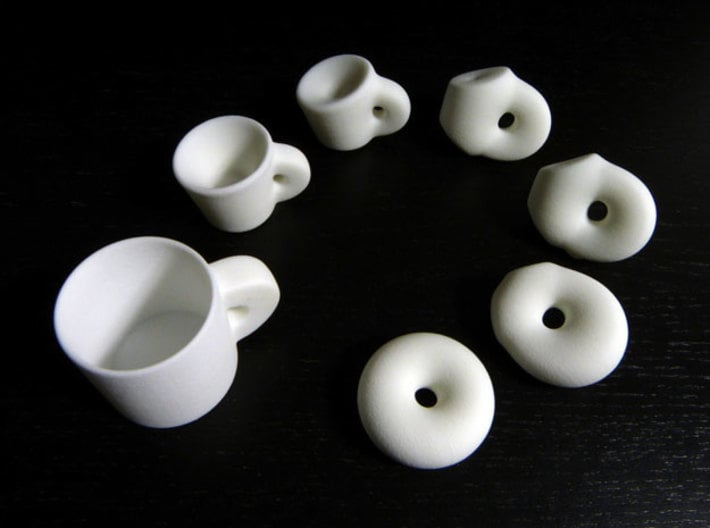
\includegraphics[scale=0.5]{coffee-mug-to-donut}
        \caption{Deformation of a coffee mug to donut}
    \end{figure}
    \item The closed disk $\{(x,y) \in \RR^2 \mid x^2 + y^2 \le 1\}$ is homeomorphic to the closed square $[-1,1] \times [-1,1]$. Intuitively, the disk can be turned into the square by stretching.
    \item In the same manner, the unit circle $S^1 = \{(x,y) \in \RR^2 \mid x^2 + y^2 = 1\}$ and a square $T = \{(x,y) \in \RR^2 \mid |x| + |y| = 1\}$ are the same. Since there is function $f : S^1 \lra T$ defined by
    \[
        f(x,y) = \left(\frac{x}{|x| + |y|}, \frac{y}{|x| + |y|}\right)  
    \]
    which is continuous, open and bijective.
    \item Let $a,b \in \RR$ with $a < b$. Define $f: [0,1] \lra [a,b]$ by 
    \[
        f(t) = (1-t)a + tb 
    \]
    $t \in [0,1]$. Then $f$ is continuous, one-to-one and onto. Its inverse is given by 
    \[
        f^{-1} (u) = \frac{u-a}{b-a}  
    \]
    $u \in [a,b]$, which is also continuous. Hence $f$ is a homeomorphism and the spaces $[0,1]$ and $[a,b]$ are homeomorphic.

\end{enumerate}

\begin{defn} 
    Let $X$ be a topological space.
    \begin{enumerate}
        \item A class $\{G_i\}$ of open subsets of $X$ is said to be an open cover of $X$ if each point of $X$ belongs to at least one $G_i$. That is, $\{G_i\}$, a collection of open sets is a cover for $X$, if $X = \cup_{i \in I} G_i$.
        \item A subclass of an open cover of $X$ which itself is an open cove is called a \textit{subcover}.
        \item An open cover (or subcover) is \textit{finite} if it contains finitely many elements.
    \end{enumerate}
\end{defn}

\begin{defn}[Compact space]
    A compact space is a topological space $X$ in which every open cover $\{G_i\}_{i \in I}$ of $X$ has a finite subcover. That is, there exists $G_1, \ldots, G_n \in \{G_i\}_{i \in I}$ so that $X  = G_1 \cup \ldots \cup G_n$ 
\end{defn}

\begin{defn}
    A topological space $X$ is called a $T_0$ space if given any pair of distinct points $x \neq y$ in $X$, there is a neighborhood $U \subset X$ satisfying $x \in U$ and $y \notin U$ or there is a neighbourhood $U \subset X$ satisfying $x \notin U$ and $y \in U$.

    That is, given any pair of distinct points in $X$, there exists a neighbourhood containing one of the points but not the other. This property is called the \textit{zeroth separation axiom.} 
\end{defn}

\begin{defn}
    A topological space $X$ is a $T_1$ space or satisfies the \textit{first separation axiom} if given an pair of distinct points, each has a neighbourhood which doesnot contain the othher. That is, for all $x,y \in X. \, x \neq y$ there exist neighbourhoods $U_x, U_y$ suchh that $x \in U_x, \, y \notin U_x$ and $y \in U_y, \, x \notin U_y$.

    A $T_1$ space is sometimes called \textit{Fr\'echet space} 
\end{defn}

\begin{defn}[Hausdorff Space]
    An Hausdorf space or $T_2$ space is a topological space in which each pair of distinct points can be separated by open sets in the sense that the points have disjoint neighbourhoods.
\end{defn}

\begin{defn}[Regular space]
    A topological space $X$ is said to be regular if it has the property that if $x \in X$ and $F$ any closed subspace of $X$ such that $x \notin F$, there exists disjoint open sets $U,V$ such that $F \subset U$ and $x \in V$. That is, it is always possible to separate $x$ and $F$ with disjoint open sets, when $x \notin F$.
\end{defn}

\begin{prop}
    Every subspace of a regular space is regular.
\end{prop}

\begin{proof}
    Let $(X, \tau)$ be a regular space and $(Y, \tau_Y)$ be its subspace. Let $x$ be a poit in $Y$ and $F$ a $\tau_Y$ closed subset of $Y$ not containing $x$. Then there is a closed subset $G$ of $X$ such that $F  = G \cap Y$. Since $x \notin G$ and $X$ is regular there are disjoint $\tau$-open sets $U, V$ such that $x \in U$ and $F \subseteq V$. Then $Y \cap U$ and $Y \cap V$ are disjoint $\tau_Y$ open sets with $x \in Y \cap U$ and $F \subseteq Y \cap V$. Thus, $(Y, \tau_Y)$ is regular.
\end{proof}

\begin{defn}
    Let $X$ be a topological space 
    \begin{enumerate}
        \item A separation of $X$ is a pair $U,V$ of open subsets of $X$ whose union is $X$.
        \item $X$ is said to be connected if it cannot be represented as the union of two disjoints open sets. That is there doesnot exist a separation of $X$.
    \end{enumerate}
\end{defn}

\begin{defn}[Path]
    Given any points $x,y$ in a topological space $X$, a path in $X$ from $x$ to $y$ is a continuous function $\alpha : [0,1] \lra X$ with $\alpha(0) = x$ and $\alpha(1) = y$, since we can rescale it to $\beta(t) = \alpha((b-a)t + a)$ for $t \in [0,1]$
\end{defn}
\begin{defn}[Path-connectedness]
    A path connected space is a topological space $X$ in which for any points $x,y \in X$ there exists a path in $X$ from $x$ to $y$.
\end{defn}

\begin{defn}[Homotopy]
Let $X$ and $Y$ be two topological spaces, let $f,g : X \lra Y$ be maps and $I = [0,1]$. Then the \textit{homotopy} from $f$ to $g$ is the map $F: X \times I \lra Y$ such that $F(x,0) = f(x)$ and $F(x,1) = g(x)$ for all points $x \in X$.
\end{defn}

\begin{notn}
If $F$ is the homotopy from $f$ to $g$ we write $\disp f \htp{F} g.$
\end{notn}

If in addition, $f$ and $g$ agree on some subset $A$ of $X$, we may wish to deform $f$ to $g$ without altering the values of $f$ on $A$. IN this particular case, we define an homotopy $F$ from $f$ to $g$ with the additional property that 
\[
    F(a,t) = f(a) \quad \text{for all $a \in A$, and all $t \in I = [0,1]$}  
\]
when such homotopy exists we say that $f$ is homotopic to $g$ relative to $A$.

\begin{notn}
    If $F$ is the homotopy from $f$ to $g$ relative to $A$ we write $\disp f \htp{F} g \rel A.$
\end{notn}

\begin{lem}
    The relation of homotopy is an equivalence relation on the set of all maps from $X$ to $Y$.
\end{lem}
\begin{proof}
    Let $f,g,h$ be maps from $X$ to $Y$. For any $f$ we have $f \htp{F} f$ where $F(x,t) = f(x)$, so the relation is reflexive. Also if $f \htp{F} g$ then $g \htp{G} f$ where $G(x,t) = F(x, 1-t)$, giving the symmetric property of the relation.
    \\
    Finally, if $f \htp{F} g$ and $g \htp{G} h$, then $f \htp{H} h$ where $H$ is defined by
    \begin{equation*}
        H(x,t) = \begin{cases}
            F(x, 2t) & 0 \le t \le \frac12 \\
            G(x, 2t - 1) & \frac12 \le t \le 1
        \end{cases}
    \end{equation*}
    so the relation is transitive.
\end{proof}


%%%TODO State and proof the result on the behaviour of homotopy with respect to composition of maps

\begin{defn}[Homotopy Type]
Two spaces $X$ and $Y$ have the same homotopy type (or are homotopy equivalent, or homotopic), if there exists maps $f: X \lra Y$ and $g : Y \lra X$ such that $g \circ f \simeq 1_X$ and $f \circ g \simeq 1_X$
\end{defn}


\begin{center}
    \begin{tikzcd}
        X \arrow[r, bend left=50]
        \arrow[r, leftarrow,bend right=50]
        & Y
        \end{tikzcd}
\end{center}


\subsection*{Examples of Homotopic spaces}
\begin{enumerate}
\item All homeomorphic spaces are homotopic.
\begin{figure}[H]
    \centering
    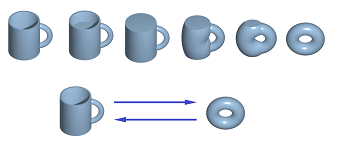
\includegraphics[scale=1]{mug-and-donut-homotopy-equivalence}
    \caption{Deformation of a coffee mug to donut showing the equivalence of both subspace of $\RR^3$}
\end{figure}
\item Any convex subset of a Euclidean space is homotopic to a point.
\end{enumerate}


%%%TODO show that homotopy type is an equavalence relation.

\begin{defn}[Contractible space]
A space $X$ is called contractible if the identity map $1_X$ is homotopic to the constant map at some point of $X$.
\end{defn}

\section{Manifolds}
Before we give the definition of what a configuration space is we give some exposition of manifolds.
\begin{defn}[Manifold\cite{lavalle2006planning}]
    A topological space $M \subseteq \RR^m$ is a \textit{manifold} if for every $x \in M$, there exists an open set $O \subset M$ such that 
    \begin{enumerate}
        \item $x \in O$
        \item $O$ is homeomorphic to $\RR^n$
        \item $n$ is fixed for all $x \in M$
    \end{enumerate}
    The fixed $n$ is called the dimension of the manifold.
    \begin{figure}[H]
        \centering
        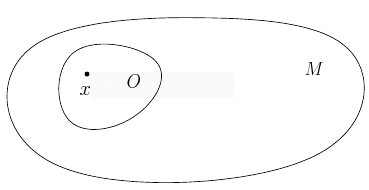
\includegraphics[scale=.95]{manifold}
    \end{figure}
\end{defn}

From the above definition, it is obvious that $m \ge n$ and it is impossible for a manifold to include its boundary points since they are not contained in open sets.
\linebreak
A manifold with boundary can be defined requiring that the neighborhood of each boundary point of $M$ is homeomorphic to a half-space of dimension $n$ and the interior points must be homeomorphic to $\RR^n$.

Now, we give presentation on the construction of some basic manifolds that frequently appear in motion planning.

\subsection{Examples of manifolds}

\begin{enumerate}
    \item \textbf{$1D$ manifolds}: A very obvious example of a one dimensional manifold is $\RR$, since by homeomorphism $\RR$ looks like $\RR$ in the vicinity of every point. The range can be restricted to the unit interval to yield the manifold $(0,1)$ since they are homeomorphic.

    Another example of a $1D$ manifold is a circle, say $\Sb^1$, where
    \[
        \Sb^1 = \{(x,y) \in \RR^2 \mid x^2 + y^2  = 1\}
    \]
    \item \textbf{$2D$ manifolds}: Many important $2D$ manifolds can be formed by applying cartesian product to $1D$ manifolds. 
    \begin{itemize}
        \item The $2D$ manifold $\RR^2$ is formed by $\RR \times \RR$ 
        \item The product $\RR \times \Sb^1$ defines a manifold that is equivalent to an infinite cylinder
        \item Also, $\Sb^1 \times \Sb^1$ is a manifold that is equivalent to a torus.
    \end{itemize}
    \begin{figure}[H]
        \centering
        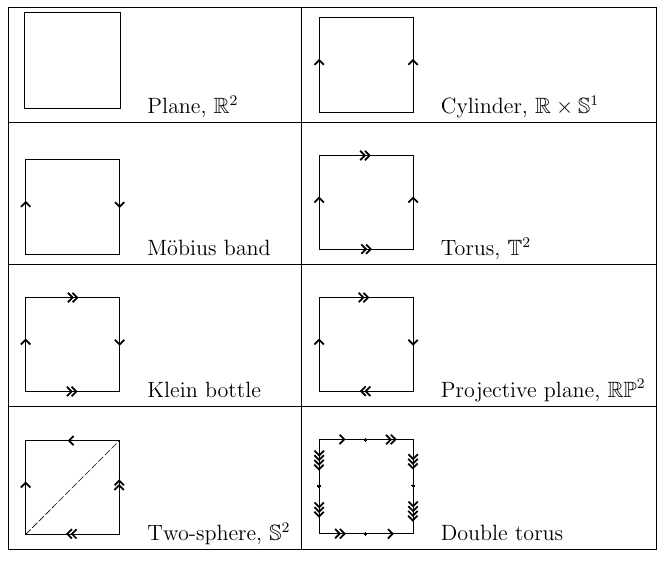
\includegraphics[scale=.85]{2d-manifolds}
        \caption{Some 2D manifolds that can be obtained by identifying pairs of points along the boundary of a square region\cite{lavalle2006planning}}
    \end{figure}
    \item 
\end{enumerate}


\section{Fundamental Group}
\begin{defn}[Loop]
    Let $X$ be a topological space and $\gamma : X \lra [0,1]$ be a continuous path in $X$. We call $\gamma$ a \textit{loop} if $\gamma(0) = \gamma(1)$.
\end{defn}

\begin{defn}[Loop]\cite{enwiki:fg}
    Let $X$ be a topological space a loop at a based at $x_0$ is the continuous path $\disp \gamma : [0,1] \lra X$ such that the starting point $\gamma(0)$ and the end point $\gamma(1)$ are both equal to $x_0$
\end{defn}

Now, let $\alpha$ be a loop and let some $x_b$ be designated as a base point. For some arbitrary but fixed basse point, $x_b$, consider the set of all loops such that $\alpha(0) = \alpha(1) = x_b$. This can be made into a group by defining the following opeartion.

Let $\tau_1 : [0,1] \ra X$ and $\tau_2 : [0,1] \ra X$ be two loop paths with the same base point. We define their product as $\tau = \tau_1 \cdot \tau_2$ and is defined as
\begin{equation}\label{eqn:fgbo}
    \tau(t) = (\tau_1 \cdot \tau_2)(t) = \begin{cases}
        \tau_1(2t) & 0 \le t < \frac12 \\
        \tau_2(2t - 1) & \frac12 \le t \le 1
    \end{cases}  
\end{equation}

This results in a continuous loop path because $\tau_1$ terminates at $x_b$, and $\tau_2$ begins at $x_b$. That is the two paths are concatenated end to end.

Suppose now that the equivalence relation induced by homotopy is applied to the set of all loop paths through a fixed point, $xb$ . It will no longer be important which particular path was chosen from a class; any representative may be used. The equivalence relation also applies when the set of loops is interpreted as a group. The group operation actually occurs over the set of equivalences of paths.

The quotient set of the set of loops illustrated above and the equivalence class of homotopy form a group with respect to the binary operation $\cdot$ defined in (\ref{eqn:fgbo}) above and its construction is illustrated below. 

The identity element is the constant loop which stays at $x_b$ for all $t \in [0,1]$, inverse of a loop is the same loop but traversed in an opposite direction. That is $\tau^{-1}(t) = \tau(1-t)$. To show associativity, consider the three loops $\tau_0, \tau_1,\tau_2$, the products $\tau_0 \cdot (\tau_1 \cdot \tau_2)$ and $(\tau_0 \cdot \tau_1) \cdot \tau_2$ is the concatenation of the loops traversing $\tau_0$ to $\tau_1$ and to $\tau_2$. Though the concatenation is not in same order, but we are only considering the class upto homotopy, the loops are the same, then we have that:
\[
    (\tau_0 \cdot \tau_1) \cdot \tau_2 = \tau_0 \cdot (\tau_1 \cdot \tau_2)
\]
which shows that the quotient set of loops with base point $x_b$ with respect to the equivalence class of homotopy on $X$ is a group. Such group is called the \textit{fundamental group} of $X$ and it is denoted $\pi_1(X)$.

\subsection{Examples of Fundamental Groups}
\begin{enumerate}
  \item \textbf{Simply connected space}: Suppose that a topological $X$ is simply connected. In this case, all loop paths from a base point $x_b$  are homotopic, resulting in one equivalence class. The result is $\pi_1(X) = 1_G$, which is the group that consists of only the identity element\dots

  \item \textbf{The Fundamental group of a Circle}: Suppose $X = \Sb^1$. In this case, there is an equvalence class of paths for each $i \in \ZZ$, if $i > 0$, then it means  that the path winds $i$ times around $\Sb^1$ in the counterclockwise direction and then returns to $x_b$. If $i < 0$, then the path winds around $i$ times in the clockwise direction. If $i = 0$, then the path is equivalent to the one that remains at $x_b$. The fundamental group is $\ZZ$, with respect to the operation of addition. If $\tau_1$ travels $i_1$ times counterclockwise, and $\tau_2$ travels $i_2$ times counterclockwise, then $\tau = \tau_1 \cdot \tau_2$ belongs to the class of loops that travel around $i_1 + i_2$ times counterclockwise. Now to consider additive inverses, suppose a path travels ten times around $\Sb^1$, and it is combined with a path that travels ten times in the opposite direction, the result is homotopic to a path that remains at $x_b$. Thus, we have that $\pi_1(\Sb^2) = \ZZ$.
  \item \textbf{The fundamental group of Torus, $\TT$:} For the torus, $\pi_1(\TT^n) = \ZZ^n$, in which the $i$th component of $\TT^n$. The fundamental group $\ZZ^n$ is obtained by starting with a simply connected subset of the plane  and drilling out $n$ disjoint, bounded holes.
    \begin{figure}[H]
      \begin{center}
        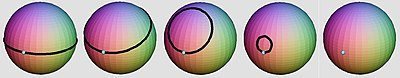
\includegraphics[width=0.85\textwidth]{sphere-homo}
      \end{center}
      \caption{A loop on a $2$-sphere (the surface of a ball) beiing contracted to a point \cite{enwiki:fg}
}
    \end{figure}
\end{enumerate}
The table below gives a summary of some space and the fundaental groups.
\begin{table}[H]
  \centering
  \begin{tabular}{c|c}
    \hline
    Space & Fundamenta group \\
    \hline 
    Convex subset of $\RR^n$ & Trivial \\
    Circle & $\ZZ$ \\
    $\Sb^n, n \ge 2$ & Trivial \\
    Torus ($\TT^n$) & $\ZZ^n$ \\
    Klein bottle & $\{a, b \mid a^2 = b^2\}$
    \end{tabular}
\end{table}

More generally we give the following definition:

\begin{defn}
   Let $X$ be a patrh-connected topological space, and $n$ a fixed integer. The $n$-homotopy group of $X$ is defined to be 
   \[  
      \pi_n(X) := 
   \]
\end{defn}

\section{Configuration Space}
There is no way we can discuss the application of topology to robotics without discussing the configuration space, since that is the entry point of topology into the field of robotics.
